\section{Experiments}
\label{sec:pending-studies}
\label{sec:evidence}
The experiments follow the distinction between a predictor, an action class and a registration. We first establish what fitted maps predict and which simpler explanations compete with them. We then measure exact-action costs on complete banks, evaluate the transfer of a particular constructed action, and compare coherent registrations. A final context-transport study tests the reach of a predictive fitting objective under a new language construction.

\subsection{Models, coordinate banks, and evaluation design}
\label{sec:design}
We analyze six frozen, pretrained decoder-only autoregressive Transformers: Llama-3.2-1B/3B, Llama-3.1-8B and Qwen2.5-1.5B/3B/7B. Four normalized depth slots, $0.2,0.4,0.6,0.8$, give 24 model/readout conditions per domain. Each has its own training-derived coordinate system and operator family. The primary coordinate dimension is 16; the spectral sensitivity comparison uses the first eight coordinates of the same saved PCA. The C7/D4 states are visible input words throughout these evaluations.

The data constructions serve different purposes. The structural-recovery bank (Study~1) contains 40 short templates per domain. Each of five seeded partitions allocates 28 to training, six to diagnostic validation and six to testing, keeping all states of a template together. The coordinate bank (Study~2) uses a separate grammar construction with 48 training, 16 validation and 64 test families, each comprising two paired variants and complete state sets. Its test bank therefore contains 128 complete state blocks per condition. Those blocks support both predictor evaluation and the finite-bank spectral calculation, with different losses. A further 64-family authored bank is reserved for the context-transport comparison.

\hypertarget{par:estimation}{}
Study~1 ridge fits no-intercept maps with coefficient $0.01$. Joint starts from these maps and uses AdamW to optimize the small matrices with soft prediction and algebraic penalties; the language model stays frozen. Generator-only fitting withholds supervision for nongenerator elements. Study~2 uses the recorded training and validation rules for each predictor, and all transfer evaluations keep their fitted coordinates fixed. For class-risk analysis, by contrast, the evaluated bank itself defines the observation distribution and second-moment metric. Including identity elements and fixed points is part of that full-group target.

All spectral means give equal weight to the 24 conditions in a domain and dimension; the orthogonal comparison includes all 96 domain/dimension/condition units. These models and readouts form a selected panel, and Study~1's five overlapping partitions are not five independent datasets. Reported bootstrap ranges describe sensitivity under the recorded resampling scheme, rather than calibrated population coverage. In the new-context comparison the unit is a paired family, retaining its measurements across models, readouts and domains together. Counts of winning conditions are descriptive panel summaries. Implementation parameters, prompts, partitions and historical resampling rules are collected in \cref{app:methods}; the Study~2 banks and follow-up designs, including paired-family resampling, are documented in \cref{app:characterization,app:pending-protocols}.

\subsection{Predictive recovery and competing explanations}
\label{sec:characterization}
\paragraph{Shared maps predict familiar transformations.}
Independent ridge predicts held-out Study~1 representations with mean $\Eeq=0.04830$ for C7 and $0.05200$ for D4. Joint yields $0.04934$ and $0.05286$: encouraging group structure does not improve this direct-prediction endpoint. It does reduce the recorded relation defects, which test generator powers and inverse/composition relations. Predictive fit and algebraic consistency can therefore respond differently to the objective, while remaining mathematically coupled through prediction residuals and operator norms.

With only generator supervision, matrix products predict five excluded nonidentity elements in each group. Their errors are $0.074443/0.056558$ for C7/D4; directly fitting those same elements in that comparison gives $0.051124/0.050032$. This is transfer across the requested action, as well as across held-out templates, but not across an unseen state vocabulary. It establishes useful predictive composition without requiring that the fitted family be an exact action. Detailed structural endpoints are in \cref{app:results}.

\paragraph{Category information provides a competitive explanation.}
The two-model lexical comparison gives near-exact fits for lexical embeddings and larger errors for internal representations at matched training projected ranks $q=6/3$. This is consistent with the finite-orbit result: generic category vectors already support every state permutation. Equal projected rank does not equalize the amount or kind of retained information.

A stronger Study~2 control makes category information explicit. It decodes the source state by its nearest training centroid and shifts the source by the difference between target and source centroids. In the equal-action compact comparison, its mean losses are $0.012013/0.063821$, versus ridge's $0.014897/0.041919$. The centroid predictor wins in 9/24 C7 and 2/24 D4 conditions: its better weekday mean is not a uniform improvement. It receives construction state labels and the exact action table, which the source-coordinate/action predictors do not. Its competitiveness demonstrates an available predictive explanation under extra information, rather than a matched-supervision victory over ridge.

Capacity also changes the comparison. Random Fourier feature (RFF) and Nystr\"om predictors fit the target-minus-source displacement from all construction target pairs, then add it to the source. Neither improves both domain means at the linear storage budget with the identity map omitted from storage; Nystr\"om does at $2\times$ storage and RFF at $4\times$. This budget counts predictor parameters, features, normalizers and lookup data, excluding shared PCA, model weights and runtime memory. The result is a ranking under stated information and storage conditions, not universal linear superiority. Nor does nonlinear predictive accuracy establish a nonlinear group action. The complete budget curves and comparator definitions are in \cref{app:reproduction}.

\paragraph{A coherent alternative survives a different control.}
Corrupting training correspondences and refitting ridge worsens prediction of the unchanged true test targets. That shows dependence on supervision. Conjugating the action by a fixed state-label swap instead defines another consistent task, preserving group laws and fixed-point counts. Ridge losses for specified/alternative correspondences are $0.014897/0.017503$ for C7 and $0.041919/0.041871$ for D4. They use the same source bank but different targets and registration-specific changed-state masks. The alternative's competitive prediction motivates asking how exceptional the prescribed action is among \emph{all} images in the declared comparator class. The original disruption and coherent-action controls are detailed in \cref{app:predictive-controls,app:reproduction}.

These comparisons concern fitted predictors. They lead to a different question: what error is unavoidable for any exact orthogonal action in the same retained space? An algebraic penalty or a competitive category baseline cannot answer that class-level question.

\subsection{Exact-action cost in observed representation banks}
\label{sec:observed-risk}
% Presentation only: select and round previously saved means.
\begin{table*}[t]
\centering\small
\setlength{\tabcolsep}{4pt}
\textbf{(a) Joint constraint cost, $r=16$}\par\smallskip
\begin{tabular}{@{}lrrrr@{}}
\toprule
Domain & Mean $\eta$ & Mean $L^\star$ bounds & Mean $L^\star-\eta$ bounds & Mean $L(I)$ \\
\midrule
$C_7$ & 0.02563 & [0.02980, 0.05863] & [0.00416, 0.03300] & 0.76012 \\
$D_4$ & 0.10321 & [0.12944, 0.24895] & [0.02624, 0.14574] & 0.52932 \\
\bottomrule
\end{tabular}
\par\medskip
\textbf{(b) Independent orthogonality and further group-law cost}\par\smallskip
\begin{tabular}{@{}rlrrrr@{}}
\toprule
$r$ & Domain & Mean $L_{\rm orth}$ & Mean $\beta$ & Mean $L^\star-L_{\rm orth}$ bounds & $\ell^->\tau$ \\
\midrule
16 & $C_7$ & 0.028706 & 0.003074 & [0.001097, 0.029927] & 23/24 \\
16 & $D_4$ & 0.127737 & 0.024531 & [0.001842, 0.121209] & 23/24 \\
8 & $C_7$ & 0.096717 & 0.029571 & [0.035397, 0.151842] & 22/24 \\
8 & $D_4$ & 0.080819 & 0.010217 & [0.000052, 0.076930] & 19/24 \\
\bottomrule
\end{tabular}
\caption{\textbf{Same-bank risks and constraint costs.} Each row averages all 24 fixed model/readout conditions on the Study~2 test banks. Panel (a) bounds the joint cost of exact laws and orthogonality; panel (b) separates the computed orthogonality cost $\beta$ from bounds on further common-law cost. Endpoints are computed per condition before averaging. The last column uses the fixed tolerance $\tau=10^{-8}+10^{-7}|\ell^-|$. Intervals bound mean class optima; they are not confidence intervals or measured optima. Each dimension uses its own second-moment-whitened metric.}
\label{tab:core-risk-summary}
\end{table*}

\begin{figure}[t]
\centering
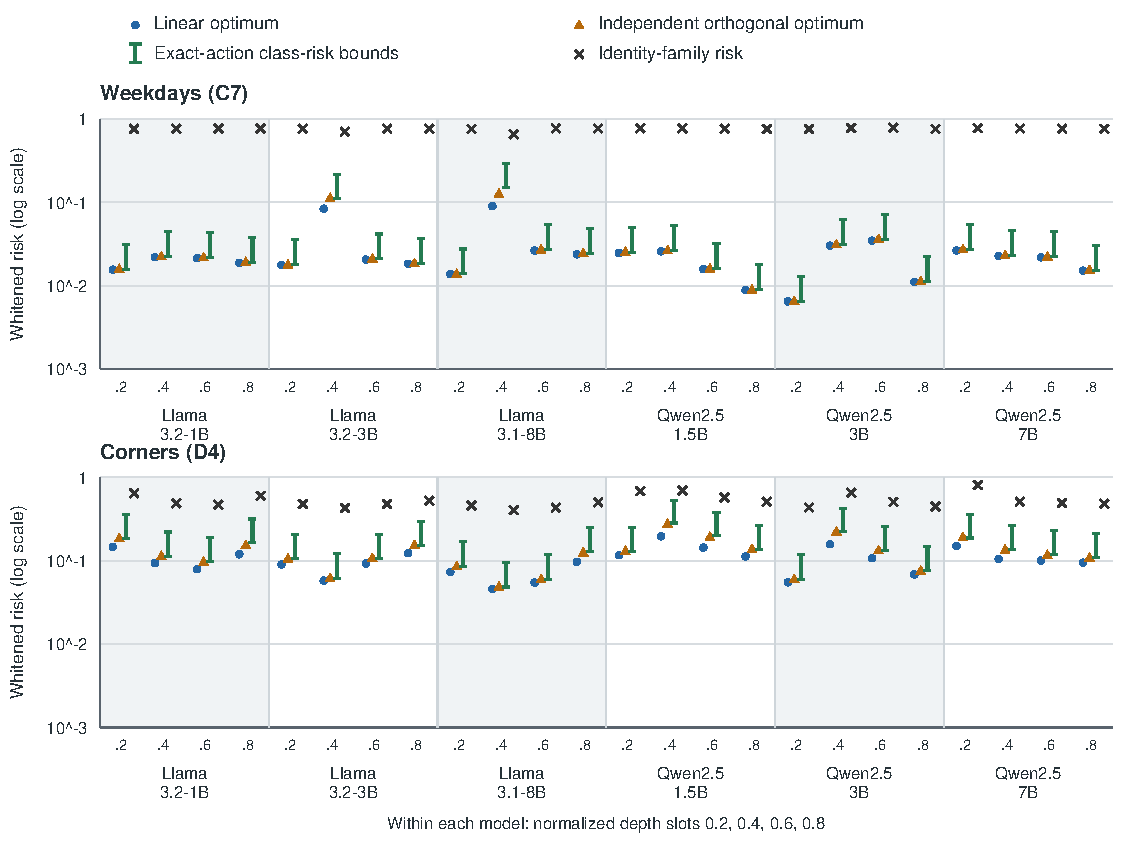
\includegraphics[width=\textwidth]{figures/same_metric_risks_v061.pdf}
\caption{\textbf{Same-metric risks in every primary condition.} Circles show $\eta$, triangles $L_{\rm orth}$, green segments $[2(1-\gamma_r),2(1-\gamma_r^2)]$, and crosses $L(I)$ at $r=16$. Within each of the 48 conditions, all four quantities use the same complete Study~2 test bank, its own second-moment whitening, and uniform state/group weights. Each model has four readouts; horizontal offsets separate symbols. The logarithmic axis shows absolute risk levels, not additive constraint costs. Segments bound the exact-action class optimum; they are neither confidence intervals nor measured witness losses. All conditions are retained. Training-metric witness transfer is reported separately in \cref{sec:witness-transfer}.}
\label{fig:same-metric-risks}
\end{figure}
We evaluate the class-risk quantities on the complete Study~2 test banks, using each bank's own empirical second moment. These are deterministic characterizations of the observed distributions, not held-out scores of training-fitted predictors. At $r=16$, the bounds support substantially better prediction than the identity-family reference on average, while quantifying a cost relative to unconstrained linear prediction (Table~\ref{tab:core-risk-summary}a). \Cref{fig:same-metric-risks} shows both comparisons in every primary condition. The absolute risks vary across models and readouts; additive costs must be read from the same-metric decomposition, rather than from distances on the logarithmic axis.

\paragraph{Orthogonality and further common-law cost.}
\label{par:orthogonal-results}
The independent orthogonal comparison separates the computed cost $\beta$ from bounds on the further cost $L^\star-L_{\rm orth}$ (Table~\ref{tab:core-risk-summary}b). At $r=16$, the latter's lower endpoint exceeds the fixed numerical tolerance in 23/24 conditions per domain. Under the stated assumptions and numerical checks, orthogonality alone therefore cannot explain the whole joint cost in those conditions. This is a bound on the remaining cost, not its exact value.

At $r=8$, the corresponding counts are 22/24 for C7 and 19/24 for D4; one C7 endpoint is only $1.55$ times its tolerance. All nine zero endpoints across both dimensions remain included. A zero lower endpoint is inconclusive about strict positivity. Each dimension has its own coordinates, whitening and normalization, so the comparison characterizes dependence on the retained space rather than selecting a superior dimension. Per-condition results and numerical rules are in \cref{app:orthogonal-results}.

\paragraph{The guaranteed costs are heterogeneous.}
At $r=16$, C7's joint-cost lower endpoints $p^-$ have median $0.000389$ and range $[0.0000349,0.06254]$. Two conditions---Llama-3.1-8B/layer 13 and Llama-3.2-3B/layer 11---contribute $90.7\%$ of their sum. D4's corresponding median is $0.01876$, with range $[0.00254,0.08719]$. All conditions retain equal weight. Moreover, positivity of $p^-$ follows from $\eta>0$ under the theorem; the data inform its magnitude and distribution, not a separate positivity discovery.

The further-law lower endpoints $\ell^-$ are even more uneven in C7: their median is $5.35\times10^{-6}$ and range $[0,0.026188]$, with Llama-3.1-8B/layer 13 supplying $99.44\%$ of the sum. This one-condition concentration concerns the further-law bound, whereas the two-condition $90.7\%$ concentration concerns the joint bound. Neither is a proportion of the unknown true costs. D4's further-law endpoints have median $0.000339$ and range $[0,0.012617]$. The upper bounds remain much wider, so small lower endpoints do not establish small actual costs.

\paragraph{Sensitivity to individual context families.}
We delete each of the 64 complete C7 families in every $r=16$ condition, removing both variants and their complete seven-state blocks together. All 1,536 deletions are evaluable, and the same 23/24 conditions exceed the original tolerance after every deletion. Llama-3.1-8B/layer 13 retains $\ell^-\in[0.02435,0.02696]$, compared with $0.02619$ on the complete bank, and accounts for $99.38\%$--$99.48\%$ of the lower-endpoint sum. Thus both the positive-bound count and the cross-condition concentration persist across these deletions. PCA remains fixed, but each reduced bank uses its own second-moment whitening: this is sensitivity to the changed empirical distribution and metric, not additive family attribution under a fixed loss. The check does not address joint deletions or shared construction biases (\cref{app:c7-family-influence}).

\paragraph{High budgets do not require a semantic computation.}
The selected trivial contributions average $b_{\rm triv}=0.61540/0.72742$: much of the captured energy is invariant to the state action. These are fractions of total whitened energy, not fractions of $\gamma_r$, and need not equal the total trivial energy used by $L(I)$. Invariant components may include contextual or constant structure; state-dependent components can still encode categories. The type correction is also small in most primary conditions: its absolute value is at most $5.33\times10^{-15}$ in 47/48. Only Llama-3.1-8B/C7/layer 13 has a material correction, $\Delta_{\rm type}/16=0.00827$. Thus real-type constraints are essential to the theorem, but their empirical effect at dimension 16 is concentrated. The detailed type decomposition is in \cref{app:bounded-risk-details}.

\subsection{Transfer of constructed exact actions}
\label{sec:witness-transfer}
\begin{table}[t]
\centering\small
\begin{tabular}{@{}lrrrrr@{}}
\toprule
& Construction bank & \multicolumn{3}{c}{Old test bank, frozen training metric} & Witness worse \\
Domain & Witness & Witness & OLS & Ridge & than OLS \\
\midrule
$C_7$ & 0.02906 & 0.02806 & 0.02141 & 0.02141 & 24/24 \\
$D_4$ & 0.11996 & 0.11117 & 0.08878 & 0.08878 & 24/24 \\
\bottomrule
\end{tabular}
\caption{Transfer of frozen predictors at $r=16$ in the training metric. These means use training whitening for both construction and old test banks, including identity and fixed points. OLS and ridge need not obey group laws. The witness is feasible, not claimed optimal. Its transfer loss is not checked against Table~\ref{tab:core-risk-summary}'s test-metric exact-orthogonal bounds: changing whitening can also change admissibility of the same raw-coordinate function.}
\label{tab:followup-witness}
\end{table}

The bounds concern the best member of an entire class on one bank. We next evaluate one concrete member when contexts are held out. For each condition, an exact-action witness is constructed from training contexts with training second-moment whitening, then frozen. All 48 constructions pass the specified numerical action-law and orthogonality checks, and their construction-bank risks lie within the analytic bounds under those checks. This verifies the intended construction numerically; it is not a rigorous floating-point certificate or evidence that the constructor attains the class optimum.

On the held-out bank, witness losses average $0.02806/0.11117$ for C7/D4, compared with $0.02141/0.08878$ for training-fitted OLS. The witness is worse than OLS and fixed-coefficient ridge in every condition (Table~\ref{tab:followup-witness}). Exact algebraic structure is therefore feasible here without improving this constructor's transfer performance. The ordering is empirical: class inclusion on one distribution does not force an ordering between training-fitted predictors on another.

The comparison also uses a different metric from the preceding bank bounds. Both construction and held-out witness losses retain the \emph{training} whitening, whereas Table~\ref{tab:core-risk-summary} characterizes the test bank in its \emph{own} whitening. Re-expressing the training action in test-whitened coordinates preserves its group law by conjugacy, but need not preserve orthogonality. Its transfer error consequently cannot be judged against that test-metric exact-orthogonal class interval. The constructor and coordinate-change derivation are given together in \cref{app:metric-conjugation}.

\subsection{Semantic registration and dimensional sensitivity}
\label{sec:registration-sensitivity}
The existence of a compatible action leaves open which action on state labels is preferred. We enumerate all 120 distinct cyclic order-seven permutation-image subgroups on the weekdays and all three dihedral order-eight images on the corners, including the prescribed image. These counts concern image subgroups, not choices of generators or arbitrary inconsistent relabelings. Every candidate defines coherent transformed targets on the same source bank.

At $r=16$, the prescribed image has uniquely highest $\gamma_r$ in 7/24 C7 and 16/24 D4 conditions. To interpret these ranks, we also compare absolute budgets. For the prescribed image $H_0$, let
\[
 d_{\rm top}=\gamma(H_0)-\max_{H\ne H_0}\gamma(H),\qquad
 d_{\rm median}=\gamma(H_0)-\operatorname{median}_{H\ne H_0}\gamma(H).
\]
The median strongest-alternative margin is $-5.52\times10^{-6}$ in C7 and $5.96\times10^{-6}$ in D4 (Table~\ref{tab:bounded-margins}). C7's budget spread across all images has median $3.88\times10^{-5}$ and maximum $4.07\times10^{-4}$, although its semantic rank ranges from first to a tied interval of 102--105 among 120. D4 spans all three ranks, with median spread $1.36\times10^{-4}$ and maximum $0.03984$. Rank changes can therefore accompany small absolute changes, particularly for weekdays. These are spectral-budget comparisons between registered tasks, not exact-$L^\star$ rankings, permutation $p$-values or semantic probabilities.

\begin{table}[t]
\centering\small
% Generated by analysis/main30_bounded_v1/derive.py; never edit numbers.
\begin{tabular}{llrrrc}
\toprule
Domain & Margin & Median & Min. & Max. & U/T/B \\
\midrule
C7 & $d_{\rm top}$ & $-5.52\!\times\!10^{-6}$ & $-3.03\!\times\!10^{-4}$ & $1.97\!\times\!10^{-5}$ & 7/0/17 \\
 & $d_{\rm median}$ & $1.60\!\times\!10^{-6}$ & $-4.13\!\times\!10^{-5}$ & $4.42\!\times\!10^{-5}$ &  \\
D4 & $d_{\rm top}$ & $5.96\!\times\!10^{-6}$ & $-1.23\!\times\!10^{-2}$ & $3.82\!\times\!10^{-2}$ & 16/0/8 \\
 & $d_{\rm median}$ & $1.46\!\times\!10^{-5}$ & $-2.04\!\times\!10^{-3}$ & $3.90\!\times\!10^{-2}$ &  \\
\bottomrule
\end{tabular}

\caption{Registration margins at $r=16$ in all 24 fixed conditions per domain. Positive values favor the prescribed image over the strongest or median alternative. U/T/B counts unique leading, tied leading and behind under the recorded pairwise tolerance. The margins measure spectral-budget differences between coherent target actions.}
\label{tab:bounded-margins}
\end{table}

A shared invariant component does not by itself settle this comparison. All enumerated images are transitive, so their full trivial energy $e_{\rm triv}$ is the same within a fixed bank: the invariant projection is the within-context state mean. Their selected contributions $b_{\rm triv}$ can differ because types compete for the dimension budget. Even a unique leader leaves automorphisms and stable state coding possible. The mechanism controls illustrate that distinction: both a shared-action construction and a stable-code construction have machine-scale noiseless witness loss, while the sampled contextual-orientation construction has smaller budgets. Stable coding is thus a compatible explanation, not a no-action null that a useful diagnostic must reject. These fixed constructions do not calibrate a semantic classifier (\cref{sp:transitive-trivial-energy,tab:followup-simulations}).

% Format-only selection from the completed sensitivity coverage.
\begin{table}[t]
\centering\small
\setlength{\tabcolsep}{5pt}
\begin{tabular}{@{}lrrrr@{}}
\toprule
Domain & $r$ & Mean $\gamma_r$ & Median $p^-$ & Unique leading image \\
\midrule
$C_7$ & 16 & 0.985102 & 0.000389 & 7/24 \\
$C_7$ & 8 & 0.933943 & 0.041288 & 4/24 \\
\addlinespace
$D_4$ & 16 & 0.935278 & 0.018756 & 16/24 \\
$D_4$ & 8 & 0.959581 & 0.005865 & 19/24 \\
\bottomrule
\end{tabular}
\caption{Retained-dimension sensitivity on the same complete Study~2 banks. Each row summarizes all 24 fixed conditions; $p^-$ is the lower endpoint for joint exact-law and orthogonality cost. The last column counts a uniquely highest budget for the specified semantic image among all 120 C7 or three D4 images, using the original tolerance. Eight coordinates are the leading eight saved PCA coordinates. The dimensions have different whitened metrics and normalizations; these are not optimal-dimension comparisons or significance tests.}
\label{tab:sensitivity-main}
\end{table}

Retaining eight rather than sixteen coordinates changes the answer quantitatively (Table~\ref{tab:sensitivity-main}). The prescribed image is uniquely leading in 4/24 C7 and 19/24 D4 conditions, and the C7 type correction exceeds the original comparison tolerance in eight conditions rather than one. No D4 condition exceeds it at either dimension. The lack of a uniform semantic preference persists, but the margins, costs and preferred images depend on the observation space. Each dimension has its own second-moment metric and $1/r$ normalization, so this is not a common-loss contest to choose an optimal dimension. The complete same-bank sensitivity results remain in \cref{app:spectral-dimension-sensitivity}.

\subsection{Context transport under a new language construction}
\label{sec:new-context}
\begin{table}[t]
\centering\small\setlength{\tabcolsep}{3pt}
\begin{tabular}{@{}lrrrrr@{}}
\toprule
& \multicolumn{3}{c}{Mean context-difference loss} & Difference minus & Family sensitivity \\
Panel & Identity & Coordinate fit & Difference fit & coordinate & range \\
\midrule
$C_7$ & 0.04357 & 0.05031 & 0.04448 & -0.00583 & [-0.00668, -0.00501] \\
$D_4$ & 0.16615 & 0.12273 & 0.12892 & +0.00619 & [+0.00397, +0.00841] \\
Equal-domain mean & 0.10486 & 0.08652 & 0.08670 & +0.00018 & [-0.00103, +0.00136] \\
\bottomrule
\end{tabular}
\caption{New authored contexts under matched validation selection. Losses use old-training difference energy. Negative contrasts favor difference fitting. The last column copies the recorded 2.5th/97.5th percentiles from 2,000 paired-family bootstrap draws; it describes conditional sensitivity over 64 authored families, not calibrated population coverage. Model/readout cells and both domains remain paired in each family.}
\label{tab:followup-context}
\end{table}

A separate prediction question is whether an objective that helps within one context construction also helps on new wording. For paired variants $v=0,1$ of a context family $f$, define $u_{i,f}=z_{i,f,0}-z_{i,f,1}$ and its transformed target $u_{g(i),f}$. Coordinate fitting learns a map on $(z_{i,t},z_{g(i),t})$ and applies it to $u$; difference fitting learns directly from $(u_{i,f},u_{g(i),f})$. Both losses divide squared difference error by the original training difference energy $E_u$. Subtracting same-state representations cancels state-only components but retains context main effects, so the target is not a pure state--context interaction.

The new bank contains 64 assistant-authored paired frames per domain, or 896 weekday and 512 corner prompts per model. Both predictors are fitted on the original training families. Their ridge coefficients are selected using the same original-validation context-difference loss, with no fitting or selection on the new bank. The earlier coordinate comparator instead used coordinate-loss selection. A secondary arm retaining that earlier rule has the same domain signs; nevertheless, comparing the old and new primary results changes selection as well as language construction, rather than isolating language alone. This study evaluates predictive transport, not spectral risks or registration rankings on new contexts.

Difference fitting minus coordinate fitting is $-0.005833$ for C7 and $+0.006190$ for D4 on average. It improves 20/24 weekday conditions and only 8/24 corner conditions. Table~\ref{tab:followup-context} also makes the reference choice important: identity has the smallest weekday mean, while both fitted predictors improve on identity for corners. The equal-domain contrast, $+0.000178$, nearly cancels; its recorded family-resampling percentiles are $[-0.001035,+0.001362]$. Neither cancellation nor an interval spanning zero establishes equivalence. The useful answer is domain-specific: fitting differences helps relative to coordinate fitting for weekdays and hurts for corners in this authored construction.

\begin{figure}[t]
\centering
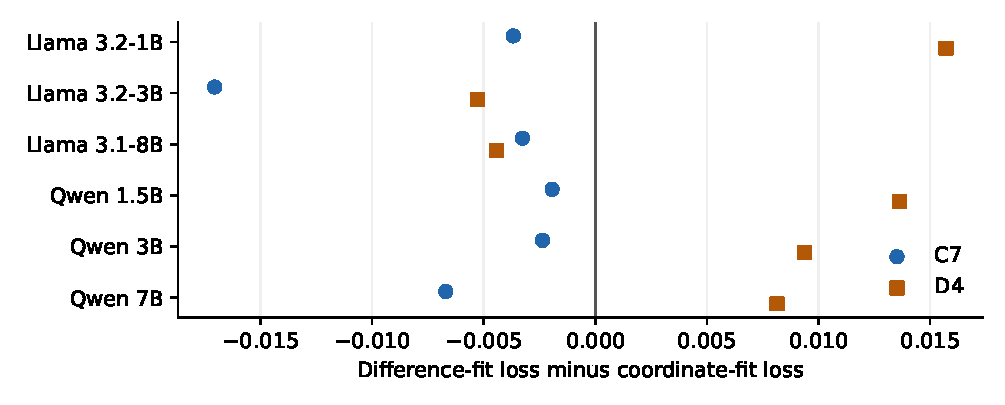
\includegraphics[width=.88\textwidth]{figures/context_transfer_followup.pdf}
\caption{New-context difference-fit minus coordinate-fit loss by model, averaged over four fixed readouts. Negative values favor difference fitting. All six weekday model means are negative, whereas four corner model means are positive. The points summarize the selected panel, not independent population draws; Table~\ref{tab:followup-context} gives the paired-family sensitivity ranges.}
\label{fig:context-followup}
\end{figure}

The frames retain the seen state vocabulary while changing outer narratives and limited factual wording. They are authored pairs, not independent human-prose samples, and only text preceding or overlapping a state span can affect its readout in a causal decoder. The reversal therefore limits a general advantage for difference fitting without identifying a native computation. The exact selection and paired-family resampling contracts are in \cref{app:pending-protocols}.
